% !TeX spellcheck = en_GB
% %%% ***************** CHAPTER INTRODUCTION ***************** %%%
\chapter{Introduction}
\label{ch:intro}
%%%%%%%%% INTRODUCTION %%%%%%%%%%%%%%
An increased frequency of extreme weather events and heat waves, droughts, heavy rains or extremely high winds is one predicted consequence of global warming \citep{hansen_warmer_2014}. Weather and climate extremes can have serious effects on human society and infrastructure, as well as on ecosystems and wildlife. Therefore, they are mostly in the media reports on the topic of climate in the focus \citep{meehl_introduction_2000}. Understanding and predicting the impact of extreme weather events is one of the major challenges of current climate research \citep{stocker_working_2013,field_summary_2014}.
% \\
% \\
\par\medskip
\noindent
It has long been known that measuring precipitation, especially in the form of snow, is difficult. Winter precipitation measurement errors between different observation networks and different regions show biases of more than \SI{100}{\percent} \citep{kochendorfer_analysis_2017}. Uncertainties in precipitation measurements under windy conditions can affect water balance calculation and the calibration of remote sensing algorithms \citep{wolff_derivation_2015}. Measurement uncertainties can be caused by the instrument itself, which varies with wind speed, wind shielding, shape and size, as well as phase and fall velocity of hydrometeors \citep{kochendorfer_analysis_2017,wolff_derivation_2015}. 
\\
Precipitation observations are important for hydrological, climate and weather research, as more than one-sixth of the world's population receives water from glaciers and seasonal snow packs \citep{barnett_potential_2005}.
\\
Since winds have an influence on solid precipitation, a WMO (World Meteorological Organization) precipitation analysis between 1987 and 1993 recommended that the double-fence inter-comparison reference should be used as a reference for snow measurements \citep{goodison_wmo_1998}. In 2010, it followed an adjustment for unshielded and single-shielded precipitation gauges. The adjustment transfer function represents a capture efficiency as a function of air temperature and wind speed to delimit the error for snowfall \citep{kochendorfer_analysis_2017,wolff_derivation_2015}.
% \\
% \\
\par\medskip
\noindent
Estimates from radar reflections derived snowfall rates are not unique. Nearly identical snowfall rates for given radar reflectivity signatures can be generated from various combinations of snowflake microphysical properties and particle fall velocity. This can lead for individual events to an error in retrieval uncertainties of \num{100}--\SI{200}{\percent} \citep{wood_estimation_2011}. \citet{kulie_utilizing_2009} used CloudSat Cloud Profiling Radar (CPR) reflectivity to estimate the global dry snowfall rate for one year. They found that snowfall estimates critically depend on assumed snowfall particle size distribution, shape and radar reflection. These studies suggest that snowfall estimates resulting only from radar reflections are ambiguous. Numerous different combinations of snowflake microphysical properties and snow particle falling rates can yield to nearly identical surface snowfall rates for a given reflectivity profile. Therefore, the use of traditional Ze-Se relationships can lead to a large difference when comparing different snowfall events \citep{cooper_variational_2017}.
\\
Based on observations of particle size distribution, fall velocity, snowflake habit, and a modified version of the optimal estimation CloudSat snowfall algorithm followed an average difference reduction to \SI{18}{\percent} of snowfall estimates, when compared to a National Weather Service measurement in Barrow, Alaska \citep{cooper_variational_2017}.
% \\
% \\
\par\medskip
\noindent
With the increasing expansion of computational power, developments of high-resolution numerical weather forecasting models with $\le$\SI{4}{\km} scales can enable small-scale phenomena such as convective dynamics to be represented \citep{gowan_validation_2018}. This enhancement provides weather services the ability to improve short-term weather forecasts for convective events, which can seriously impact infrastructure and society \citep{muller_arome-metcoop:_2017}. The ability to use high-resolution models is also followed by various challenges, such as physical parametrisation schemes, accurate representation of topography, and data assimilation of high-resolution data \citep{sun_convective-scale_2005}.
\\
The weather forecast in Scandinavia covers a wide range of phenomena and includes continental, maritime and polar conditions. Norway has a complicate coastline, gradients in land use, as well as complex topography, which can complicate local weather forecasting of temperature, wind and precipitation \citep{muller_arome-metcoop:_2017}. Several studies such as \citet{colle_1314_2005,garvert_1314_2005,schwartz_reproducing_2014} have shown, that simulations of orographic precipitation can be improved in mountainous terrain for horizontal grid spacing below \SI{4}{\km}. Uncertainties on a convective scale can lead to a rapid error growth \citep{lorenz_atmospheric_1969}, hence high-resolution ensemble prediction make it possible to estimate the forecast uncertainty by performing several model runs, each with different initial conditions. %\citep{gowan_validation_2018}
% \\
% \\
\par\medskip
\noindent
This work focuses on the measurement site Haukeliseter in Southern Norway and the extreme storm during Christmas 2016. The extreme storm was named 'Urd' by the Norwegian meteorological Institute. Storms of this kind are expected to occur on average every five years. The financial costs associated with 'Urd' are estimated to about 180 million Norwegian kroner. 'Urd' led to major traffic problems for cars, trains, ferries and air planes. Most mountain crossings were kept closed during Christmas 2016 \citep{olsen_ekstremvaerrapport._2017}. A change in temperature and therefore change of precipitation from solid to liquid followed an increase in avalanche danger. In addition, was there a power breakout of around 70.000 households and 40 emergency power stations failed during the extreme weather (\Cref{fig:news}).
%%% images from Twitter and news %%%%%%%%%%%%%%%%%%%%%%%%%%%%%%%%%%%%%
% !TeX spellcheck = en_GB
\begin{figure}[t!]
	\centering
	\begin{subfigure}[b]{0.49\textwidth}
		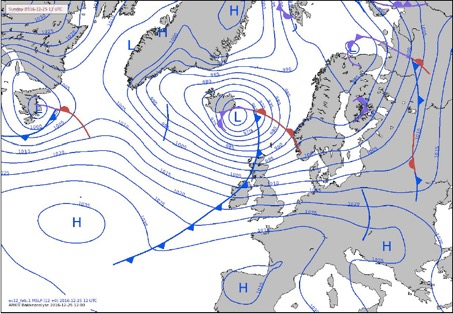
\includegraphics[width=\textwidth]{./fig_introduction/Ana_2512_12UTC.jpg}
		\caption{}\label{fig:ana_YR}
	\end{subfigure}
\hfill
	\begin{subfigure}[b]{0.49\textwidth}
		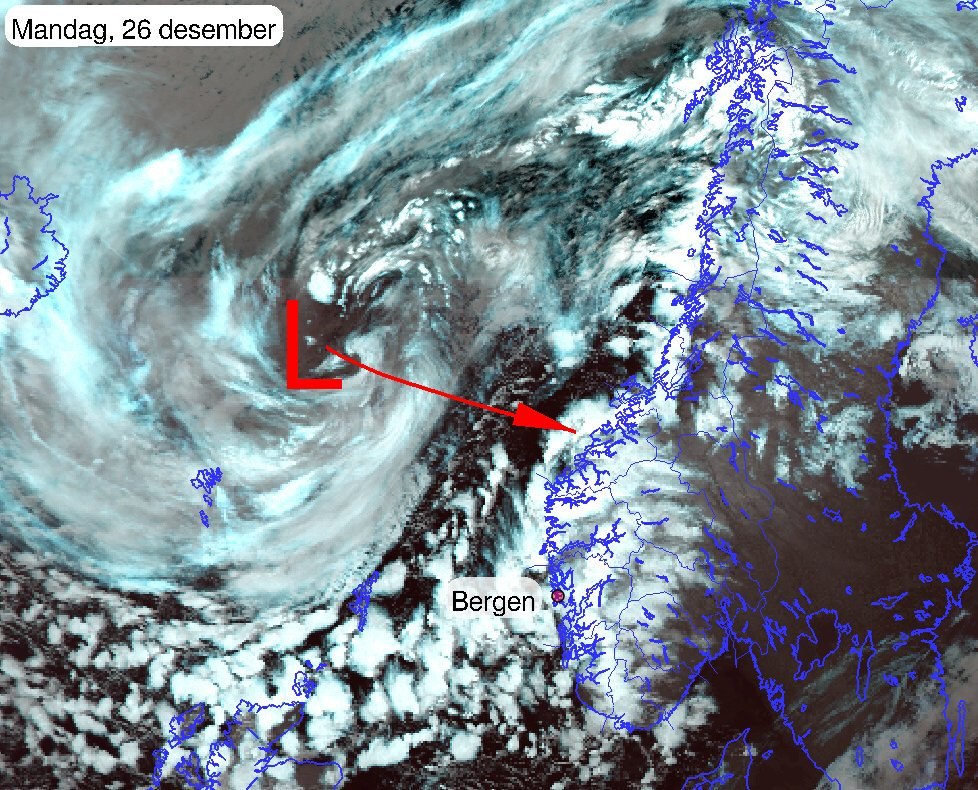
\includegraphics[trim={0cm 3.8cm 0cm 0cm},clip, width=\textwidth]{./fig_introduction/Twitter_26122016_0934AM.jpeg}
		\caption{}\label{fig:meteorologene_2612}	
	\end{subfigure}
	\begin{subfigure}[b]{0.49\textwidth}
		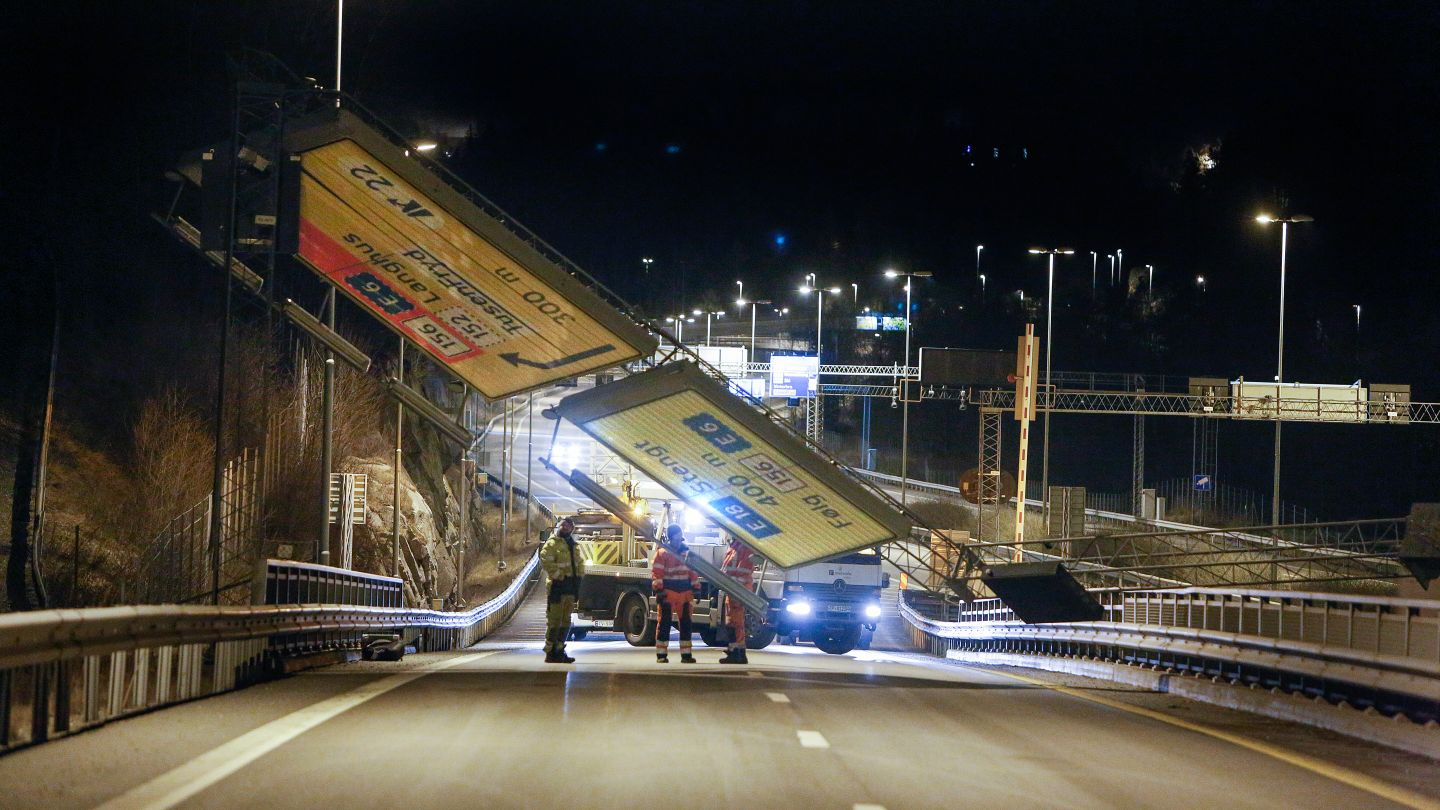
\includegraphics[width=\textwidth]{./fig_introduction/street_sign_2512.jpg}
		\caption{}\label{fig:street_sign}
	\end{subfigure}
\hfill
	\begin{subfigure}[b]{0.49\textwidth}
		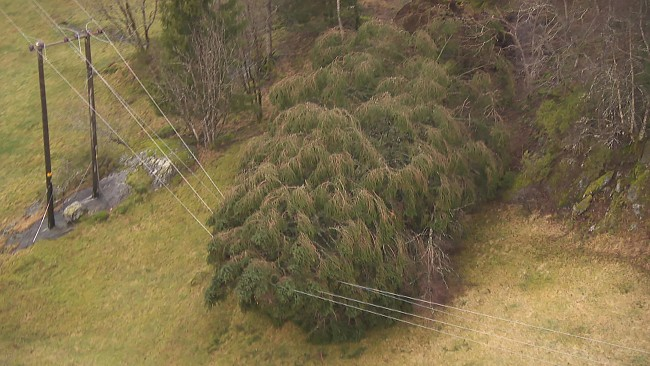
\includegraphics[width=\textwidth]{./fig_introduction/tree_nrk_2812.jpg}
		\caption{}\label{fig:tree_elec}
	\end{subfigure}
\caption{Weather situation during the extreme Christmas storm and impact on the infrastructure. In \protect\subref{fig:ana_YR}: Weather situation Sunday \SI{25}{\dec} at \SI{12}{\UTC} from the extreme weather report on Urd \citep{olsen_ekstremvaerrapport._2017}.
	\protect\subref{fig:meteorologene_2612}: Tweet from \cite{meteorologene_her_2016} on \SI{26}{\dec} at 9:34 am: Here comes \#Urd! The low pressure centre will hit M{\o}re og Romsdal, but the strongest wind comes south of Stad. \#S{\o}rNorge.
    \protect\subref{fig:street_sign} and \protect\subref{fig:tree_elec} show the consequences related to the high wind speeds during Christmas 2016.
	\protect\subref{fig:street_sign}: This traffic sign, ten meter long and four meter high was blown down during the storm, \citep{ruud_tonn_2016}.
	\protect\subref{fig:tree_elec}: Trouble maker: The extreme weather during Christmas created problems for the local infrastructure. \num{80.000} households were without electricity during the storm, \citep{farestveit_80.000_2016}.} \label{fig:news}
\end{figure}
%%%%%%%%%%%%%%%%%%%%%%%%%%%%%%%%%%%%%%%%%%%%%%%%%%%%%%%%%%%%%%%%%%%%%%%%%%
\\
The Christmas storm in 2016, might not have led to the same damages as some of the extreme weather events of recent years. But as people and infrastructure are affected by extreme weather, it is necessary to further improve the accuracy of snow-ground observations to better verify numerical weather forecasts, hydrological and climate models \citep{joos_influence_2012}. This may lead to improvements in short- and long-term predictions as well as predicting the variability of the global water balance \citep{field_changes_2012}. Changes in snow pack characteristics after severe rain on snow events can lead to severe avalanches \citep{stimberis_glide_2011} and to the formation of thick layers of ice in the snow pack or on ground \citep{putkonen_rain--snow_2003,hansen_climate_2011}. 
% \\
% \\
\par\medskip
\noindent
Since winter 2010, the site has been a WMO measuring station with single and double fence precipitation instruments. In the winter of 2016/2017, three additional state of the art radar and snowflake microphysical instrumentation were deployed which could be uset to estimate the vertical profile of snow water content in the atmosphere. The snowflake characteristics are estimated using a multi-angle snowflake camera \citep[MASC;][]{garrett_fall_2012} and a Particle Imaging Package \citep[][PiP;]{newman_presenting_2009}. With the aid of the modified CloudSat snow particle model algorithm and the snowflake properties, as well as reflectivity profiles, the amount of snowfall in the atmosphere can then be determined. The usage of a snowfall retrieval with ground-based measurements will give an insight into the microphysical structure of the extreme event. The double fence measurements should help to estimate vertically derived snowfall on the ground.
\\
Additionally, since November 2016 the Meteorological Cooperation on Operational Numerical Weather Prediction (MetCoOp) Ensemble Prediction forecast (MEPS) is operational at the Meteorological Institute of Norway (Met-Norway). The ensemble prediction system uses the previous deterministic AROME-MetCoOp, a version of the Mèteo-France Applications of Research to Operations at Mesoscale and initialises in addition ten perturbed ensemble members. The newly developed ensemble prediction systems (EPS) from Met-Norway is used to analyse the extreme winter storm during Christmas 2016. It will be shown if the ensemble prediction system is able to forecast the variation of an extreme winter storms such as 'Urd' and if it is able to predict large scale effects as well as local effects. Furthermore, the use of an ensemble prediction system will give the possibility to analyse the variation of snowfall precipitation in the vertical and at the surface. Using observations to evaluate MEPS will help to examine the following research questions. How well will the model predict the surface snowfall at the measurement site? Will precipitation transitions from snow to rain to snow forecasted by the regional model?
Does the regional model cover local affects associated with the topography around the site?
% \\
% \\
\par\medskip
\noindent
The thesis is structured as following: \Cref{ch:Methods} will give an overview of the measurement site Haukeliseter and its instrumentation. Followed by the methodology on the optimal estimation retrieval as well a description of the regional model MEPS. Afterwards the application to the data to compare the forecast system and the observations will be presented. The synoptic analysis of the extreme Christmas storm in 2016 is presented in \Cref{ch:weather_ana}. After this, will \Cref{ch:Res} present the results and the discussion on large scale effects, surface snowfall accumulation and local wind influence  at Haukeliseter. The final chapter summarises the results and findings and suggests future research which has to be done.



% One of the challenges in current forecast research is the understanding and prediction of extreme weather events, such as heavy precipitation. 
% Extreme winter storms with heavy precipitation can have large influence on the local infrastructure and the personal safety. Large amounts of precipitation combined with temperature changes can lead to danger in the Norwegians mountains. A better understanding of the microphysical processes in storms in crucial to better predict extreme storms. 
% \\
% %%%%%% into synoptic ? %%%%%
% %During Christmas 2016 an extreme storm influenced the west coast of Norway.  The storm, called 'Urd' was according to \citet{olsen_ekstremvaerrapport._2017} associated with strong winds and high precipitation amounts. 
% %The average wind along the coast of Western Norway had hurricane strength (observed: \SIrange{40}{55}{\mPs}). In South and Eastern Norway west to north-west winds between \SIrange{25}{40}{\mPs} were measured.
% %At the Haukeliseter measurement site, \SI{136.4}{\milli\metre} of precipitation were monitored during \SIrange{21}{27}{\dec}.
% %This event was just above the limit of been called an extreme weather. 
%  \citep{olsen_ekstremvaerrapport._2017}. \\ 
% 
%  
%  
% \\
%  it is important to predict storms, associated precipitation, wind, and temperature changes as accurately as possible. Having accurate observations, will lead to better performing models which rely on observations. \textcolor{red}{include a reference here}
% \newline
% \noindent
% \Cref{fig:news} shows that precipitation and strong winds can influence in certain ways the infrastructure. To predict and measure snowfall accumulation as accurately as possible is important since snowfall has impact on avalanches, freshwater release into water systems in spring, and extra economical expenses for local infrastructure as well as climatological effects. \\
% % \citet{joos_influence_2012} investigated the influence of microphysical processes on potential vorticity development in warm conveyor belts (WCB). They demonstrated the complex interaction between the small-scale microphysical processes and the large-scale flow in WCB. 
% % For the understanding of numerical simulations of storm developments, it is important to know vertical precipitation profiles and their position within the synoptic environment.% vorticity environment. 
% It is crucial to study the vertical structure of different synoptic storms and  predict as accurately as possible.\\
% % 
% Since November 2016, the Meteorological Cooperation on Operational Numerical Weather Prediction (MetCoOP) Ensemble Prediction forecast (MEPS) is operational at the Meteorological Institute of Norway (Met-Norway). The ensemble prediction system uses the previous deterministic AROME-MetCoOp, a version of the Mèteo-France Applications of Research to Operations at Mesoscale and initialises in addition ten perturbed ensemble members. The use of an ensemble prediction system will give the possibility to analyse the variation of snowfall precipitation in the vertical and at the surface.
% %The study by \citet{muller_arome-metcoop:_2017} shows that the AROME-MetCoOp performs well for certain meteorological phenomena, but that it has still some uncertainties by forecasting precipitation.  \\
% Microphysical processes in weather models are still not well understood and therefore are mostly parametrised \citep{muller_arome-metcoop:_2017}. Furthermore, high latitude regions are not well represented in meteorological models. %Indeed, a comparison between the MEPS data fit the observations for December 2016 but uncertainties are still present for this time period. 
% In this study, the newly developed ensemble prediction systems (EPS) from Met-Norway is used to analyse the extreme winter storm during Christmas 2016. It will be shown if the EPS is able to forecast the variation of an extreme winter storms such as 'Urd' and if it is able to predict large scale effects as well as local effects. 
% \\
% This work focuses on the measurement site Haukeliseter in Southern Norway. During winter 2016 state of the art ground measurements were installed to estimate the vertical snow water content in the atmosphere. The usage of a snowfall retrieval with ground-based measurements will give an insight to the microphysical structure of the extreme event. %This vertical and surface observations will help to verify the regional forecast model for a mountain side in Norway.
% \\
% Snowfall is important in the Norwegian mountains for safety and drinking water resources. The aim of this thesis is to evaluate the regional forecast model MEPS by using local observations from a mountain side in Norway. This thesis will examine research questions: How well will the model predict the surface snowfall at the measurement site? Will precipitation transitions from snow to rain to snow forecasted by the regional model?
% Does the regional model cover local affects associated with the topography around the side? 
% \\
% The thesis is structured as following: Chapter 2 will present the synoptic analysis of the extreme storm, which will later be used to evaluate MEPS. The third chapter will give an overview of the measurement site Haukeliseter and its instrumentation. Chapter 4 and 5 covers the optimal estimation snowfall retrieval and regional model, respectively. After this will Chapter 6 present the results and discussion. The daily MEPS runs will be compared to the observed surface accumulation and the vertical retrieved snow water content. Furthermore, precipitation characteristics such as wind influence and rain segments will be discussed. The final Chapter summarises the results and findings and suggests future research which has to be done. 

% %Some satellites, such as CloudSat have been equipped with radar to estimate snowfall rates and vertical profiles of precipitation. CloudSat is one of the satellites orbiting in the A-Train formation and measures the vertical structure of cloud systems \citep{stephens_cloudsat_2002}. This study is using the adapted CloudSat retrieval scheme for ground-based measurements. This will give an insight of  snowfall in the lower \SI{3}{\km} of the atmosphere. CloudSat radars are not able to observe storm structures down to \SI{3}{\km}. Using radar reflectivity from the ground can link satellite observations with ground-based observations to get a better understanding of vertical snowfall patterns.    
% % \\
% % Studies of \citet{kulie_utilizing_2009} showed that the Cloud Profiling Radar (CPR), mounted on the CloudSat, can be used to estimate global distributions of snowfall. They showed that different combinations of microphysical habits and fall speed can lead to the same results of reflectivity and therefore to the same amount of snowfall rate.
% % Methods like optimal estimation retrieval were established to reduce the non-uniqueness. Where ground observations are used to estimate vertical profiles of precipitation.\\
% % The improvement of the CloudSat retrieval is helpful to show that climate models over estimate present-day Antarctic snowfall \citep{palerme_evaluation_2017}. \citet{norin_intercomparison_2015} presented a good agreement between the ground-based snowfall measurements and satellite observations.